%%%%%%%%%%%%%%%%%%%%%%%%%%%%%%%%%%%%%%%%%
% University/School Laboratory Report
% LaTeX Template
% Version 4.0 (March 21, 2022)
%
% This template originates from:
% https://www.LaTeXTemplates.com
%
% Authors:
% Vel (vel@latextemplates.com)
% Linux and Unix Users Group at Virginia Tech Wiki
%
% License:
% CC BY-NC-SA 4.0 (https://creativecommons.org/licenses/by-nc-sa/4.0/)
%
%%%%%%%%%%%%%%%%%%%%%%%%%%%%%%%%%%%%%%%%%

%----------------------------------------------------------------------------------------
%	PACKAGES AND DOCUMENT CONFIGURATIONS
%----------------------------------------------------------------------------------------
\documentclass[
	a4paper, % Paper size, specify a4paper (A4) or letterpaper (US letter)
	12pt, % Default font size, specify 10pt, 11pt or 12pt
]{CSUniSchoolLabReport}
\usepackage[ngerman]{babel}
\usepackage{siunitx}  
\usepackage{textcase}
\usepackage{booktabs}
\usepackage[utf8]{inputenc}
\usepackage{amsmath}
\usepackage{array}
\usepackage{booktabs}
\usepackage{color}
\usepackage{tabularray}
\usepackage{pdfpages}
\sisetup{locale = DE,  
separate-uncertainty,  
range-units = brackets,  
list-units = single,  
per-mode=symbol-or-fraction,
}  
\addbibresource{sample.bib} % Bibliography file (located in the same folder as the template)
\renewcommand{\thesection}{\Alph{section}}
\renewcommand{\thesubsection}{\thesection.\arabic{subsection}}
\renewcommand{\thesubsubsection}{\thesubsection.\arabic{subsubsection}}
\newcommand{\micro}{\ensuremath{\mu}}
\newcommand{\pico}{p}
\newcommand{\milli}{m}
\newcommand{\nano}{n}
%----------------------------------------------------------------------------------------
%	REPORT INFORMATION
%----------------------------------------------------------------------------------------
\setlength{\parindent}{0pt}

\title{Protokoll Praktikum EBau Diode} % Report title

\author{Johann \textsc{Becker} \and Valentin \textsc{Eder} \and Marc \textsc{Ostner}}
\date{\today} % Date of the report

%----------------------------------------------------------------------------------------

\begin{document}


\maketitle % Insert the title, author and date using the information specified above

\begin{center}
	\begin{tabular}{l r}
		Date Performed: & 30. Mai 2025 \\ % Date the experiment was performed
		
		Instructor: & Prof. Dr. Alexandru Negut % Instructor/supervisor
	\end{tabular}
\end{center}

% If you need to include an abstract, uncomment the lines below
%\begin{abstract}
%	Abstract text
%\end{abstract}

%----------------------------------------------------------------------------------------
%	OBJECTIVE
%----------------------------------------------------------------------------------------
%A%
\section{Einführung}
Die Vorbereitung ist im Anhang zu finden.
%B%
\section{Versuchsdurchführung}
%B.1%
\subsection{Statische Messungen}
%B.1.1%
\subsubsection{Sperrschichtkapazität}
\begin{table}[ht]
\centering
\begin{longtblr}[
  label = none,
  entry = none,
]{
  width = \linewidth,
  colspec = {Q[129,c]Q[77,c]Q[119,c]Q[117,c]Q[119,c]Q[117,c]Q[77,c]Q[119,c]},
  vline{2} = {-}{},
  hline{2} = {-}{},
}
U/V  & 0     & 0,1   & 0,2   & 0,3  & 0,5  & 0,7  & 1    & 1,5  & 2  & 3,5  \\
C/pF & 122,6 & 110,1 & 102,4 & 96,5 & 87,8 & 81,6 & 74,8 & 67,2 & 62 & 52,5 
\end{longtblr}
\caption{Sperrschichtkapazitäten bei zwischen 0 bis \SI{3.5}{\volt}}
\end{table}

\begin{table}[ht]
\centering
\begin{longtblr}[
  label = none,
  entry = none,
]{
  width = \linewidth,
  colspec = {Q[129,c]Q[77,c]Q[119,c]Q[117,c]Q[119,c]Q[117,c]Q[77,c]Q[119,c]},
  vline{2} = {-}{},
  hline{2} = {-}{},
}
U/V  & 5  & 8    & 10   & 15   & 20   & 25 & 30   \\
C/pF & 47 & 40,5 & 37,7 & 33,1 & 30,1 & 28 & 26,4 
\end{longtblr}
\caption{Sperrschichtkapazitäten bei zwischen 3,5 bis \SI{30}{\volt}}

\end{table}
%B.1.2%
\subsubsection{Sperrstrom}
Absolut höchster Strom bei Diode~$\rightarrow$~Kurzschluss.
\[
U = R \cdot I \quad \Leftrightarrow \quad I = \frac{U}{R}
\]
\[
R_{Vor} = \frac{\SI{30}{\volt}}{\SI{10}{\milli\ampere}} = \SI{3}{\kilo\ohm}
\]
Die Messung muss Stromrichtig erfolgen, da durch die Sperrpolung der Diode sehr kleine Ströme zu erwarten sind. Für hohe Spannungen ist es nicht essenziell die Spannung auf den Millivolt genau einzustellen. Auch bei \SI{0.5}{\volt} ist der erwartete Strom im Verhältnis zur Spannung sehr gering. 
Das Picoampermeter wird am niederohmigen Knoten geschaltet, um den sehr kleinen Sperrstrom möglichst genau messen zu können. Dabei ist zu beachten, dass der Spannungsabfall über das Messgerät vernachlässigbar klein bleibt, damit die Messung nicht verfälscht wird.
\begin{table}[ht]
\centering
\begin{tabular}{c|cccccccccccccc}
U/\si{\volt} & 0,5 & 5 & 30\\
\hline
I/\si{\ampere} & 1\milli& 2\micro& 3\pico\\
\end{tabular}
\caption{AA136 Sperrströme bei Spannungen.}
\label{tab:uv-cf}
\end{table}


\begin{table}[ht]
\centering
\begin{tabular}{c|cccccccccccccc}
U/\si{\volt} & 0,5 & 5 & 30\\
\hline
I/\si{\ampere} & 1\milli& 2\micro& 3\pico\\
\end{tabular}
\caption{1N4002 Sperrströme bei Spannungen.}
\label{tab:uv-cf}
\end{table}
%B.1.3%
\subsubsection{Vorwärtsstrom 1N4002}

\begin{table}[H]
\centering
\begin{tabular}{c|cccccccc}
$U_R/\si{\volt}$ & 0 & 0.5 & 1 & 2 & 3 & 4 & 5 & 7.5 \\
$I/\si{\ampere}$ & 15 \nano& 30 \nano& 80 \nano& 150 \nano& 300 \nano& 800 \nano& 1.5 \micro& 3 \micro\\
\hline
$U_R/\si{\volt}$ & 10 & 12.5 & 15 & 20 & 25 & 30 & 2 & \\
$I/\si{\ampere}$ & 8\micro& 15\micro& 30\micro& 80\micro& 150\micro& 300\micro& 800\micro& \\
\end{tabular}
\caption{Sperrschichtstrom \(I/\si{\ampere}\) in Abhängigkeit von der Spannung \(U_R/\si{\volt}\).}
\label{tab:uv-cf}
\end{table}


% If you have more than one objective, uncomment the below:
%\begin{description}
%	\item[First Objective] \hfill \\
%	Objective 1 text
%	\item[Second Objective] \hfill \\
%	Objective 2 text
%\end{description}
%B.2%

\subsection{Dynamische Aufnahme von Kennlinien}
%B2.1

\subsubsection{Durchlaßkennlinien 1N4002 und AA136}
%Grafik Beginn
\begin{figure}[H] % [H] forces the figure to be placed exactly where it appears in the text
	\centering % Horizontally center the figure
	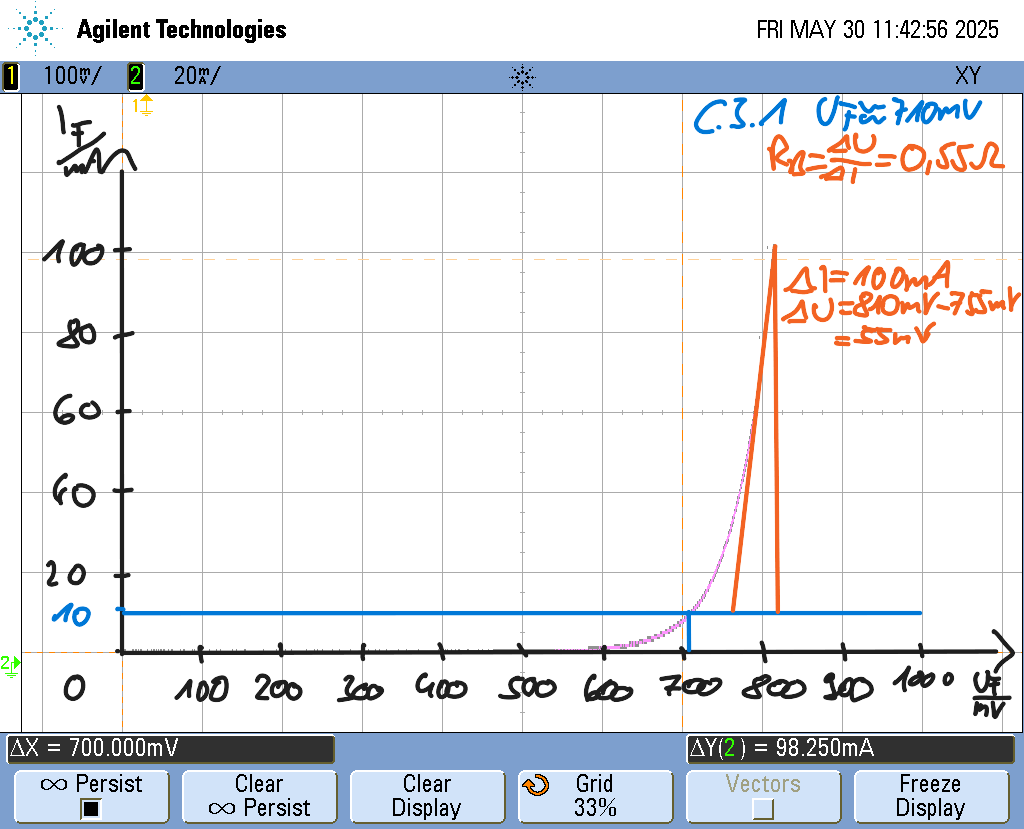
\includegraphics[width=1\textwidth]{B.2.1(1N4002)} % Include the figure, now larger
	\caption{1N4002 Durchlaßkennlinien}
\end{figure}
Bandgap 1N4002 = 3\micro m  
%newline
\\
Bandgap $A = 3/2$
%Grafik Ende
\begin{figure}[H] % [H] forces the figure to be placed exactly where it appears in the text
	\centering % Horizontally center the figure
	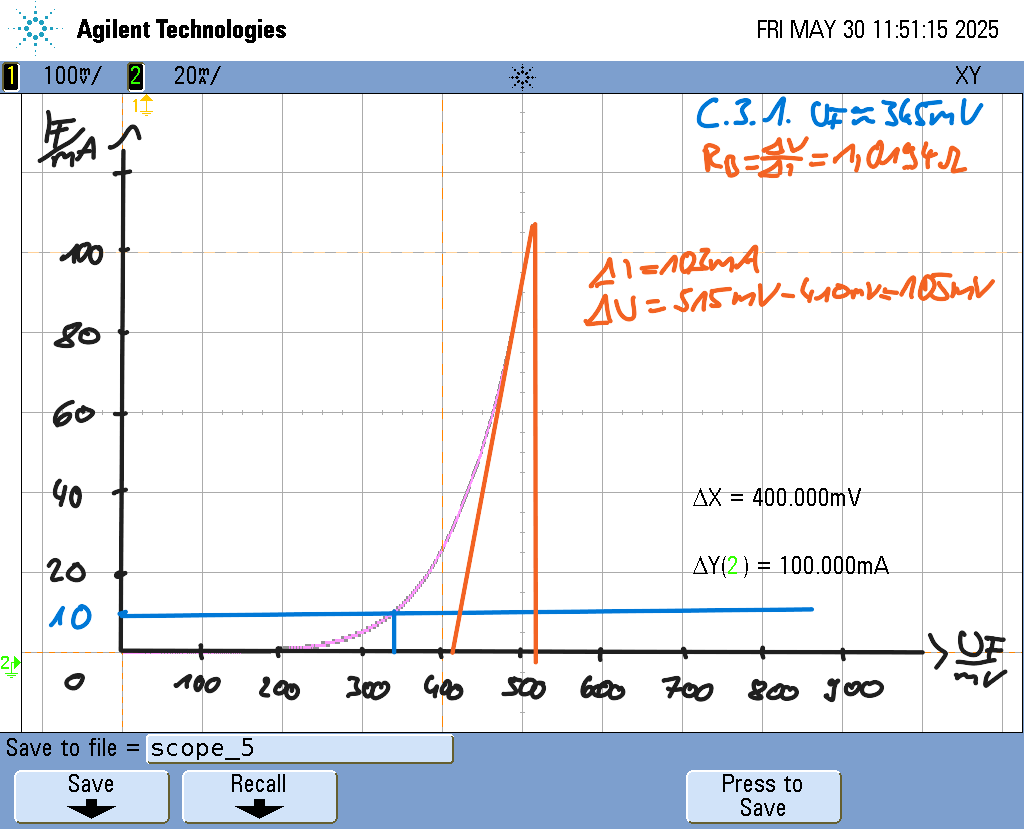
\includegraphics[width=1\textwidth]{B.2.1(AA136)} % Include the figure, now larger
	\caption{AA136 Durchlaßkennlinien}
\end{figure}

\begin{figure}[H] % [H] forces the figure to be placed exactly where it appears in the text
	\centering % Horizontally center the figure
	
\includegraphics[width=1\textwidth]{placeholder} % Include the figure, now larger
	\caption{Placeholder}
\end{figure}

\[
I_F = \frac{U_Z}{0,1 \cdot 10}
\]
$I_{F}$ 
$U_{Gen}= x$\ max.\ \SI{100}{\milli\ampere}
%B.2.2%
\subsubsection{Vergleich der Kennlinien}
\begin{figure}[H] % [H] forces the figure to be placed exactly where it appears in the text
	\centering % Horizontally center the figure
	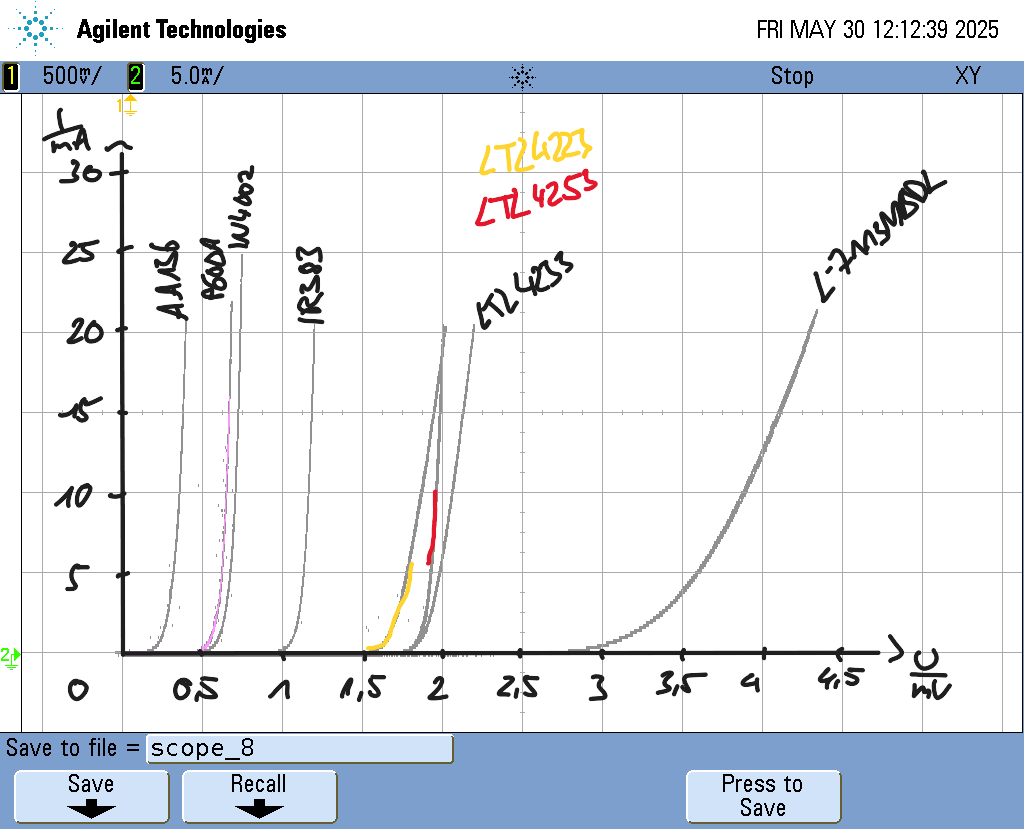
\includegraphics[width=1\textwidth]{B.2.2} % Include the figure, now larger
	\caption{Dioden Kennlinien}
\end{figure}

%B2.3.
\subsubsection{Z-Dioden}
%B.3
\subsection{Dynamisches Verhalten der Siliziumdiode (1N4002)}
%B.3.1
\subsubsection{Bestimmung von Speicher- und Abfallzeit}
%B.3.2
\subsubsection{Bestimmung der Einschaltzeiten}
$U_{pp} = 20V \quad f_{gen} = \SI{100}{\hertz}$\quad Funktion: Squarewave
%B.3.3
\subsubsection{Einfluß der Schaltzeiten auf die maximale Betriebsfrequenz}
%B.3.4
\subsubsection{Dynamische Bestimmung des Bahnwiderstands}

\[
\Delta I_D \approx \Delta U_{gen}/R \quad R_B \approx \frac{\Delta U_D}{\Delta U_{gen}/R}
\]
%C
\section{Auswertung}
%C.1
\subsection{Sperrschichtkapazität, Diffusionsspannung und \\Dotierstoffdichte}
\[
C_S = \frac{C_{S0}}{(1+\frac{U}{U_D})^M}\quad f(U) = \frac{1}{C_S^\frac{1}{M}}
\]
Stufenfaktor von x ist ein indiz für einen linearen pn-Übergang.

\vspace{1em} 

\[
% TODO: Replace 0 with the actual value 
C_{S0} = \SI{0}{\pico\farad} \quad \varepsilon _{r_{si}} = 11,7 \quad A_{RLZ} = \SI{2.5}{\milli\metre\squared}
\]
\begin{align*}
N_A &\gg N_D \rightarrow \text{abrupter pn-Übergang} \\
\rightarrow\ C_{s0} &= \sqrt{\frac{\varepsilon_r \cdot \varepsilon_0 \cdot e N_D \cdot N_A}{2 \cdot (N_D + N_A) \cdot U_D}} \cdot A_{RLZ} \\
\leftrightarrow\ N_D &= \frac{C_s^2 \cdot 2 \cdot (U_D - U)}{\varepsilon_r \cdot \varepsilon_0 \cdot A_{RLZ}^2}
\end{align*}

\vspace{1em} 
%C.2
\subsection{Vergleich verschiedener Dioden}
Für Vergleich in Übersichtsdarstellung siehe B.2.2 Grafik.
\[
\left.
\begin{array}{l}
W_g = h \cdot f \\
\lambda = \frac{c}{f}
\end{array}
\right\}
\quad \lambda = \frac{c\cdot h}{W_g} \cdot e \leftrightarrow W_g = \frac{c \cdot h}{\lambda \cdot e}
\]
Daraus folgt $\lambda = x$. \\

\[
\left.
\begin{array}{l}
I|_{U>3U_T} = I_S\cdot e^{U/U_T} \leftrightarrow U = U_T\cdot ln(\frac{I}{I_S}) \\
I_{S_{lang}} = q A n_i^2 \left( \frac{D_p}{L_p N_D} + \frac{D_n}{L_n N_A} \right) \\
n_i^2 = \sqrt{N_C N_V} \cdot \exp\left(-\frac{W_g}{2kT}\right)
\end{array}
\right\}
\quad I_s \varpropto n_i^2 \varpropto \exp\left(-\frac{W_g}{2kT}\right)
\]

\vspace{1em} 

Desto kleiner $I_s$ bzw. desto größer $W_g$, umso größer muss $U$ sein, um einen Strom $I$ zu halten.\\ \\  
Bandgaps aller Dioden aus Abbildung 4.\\
AA136 (Germanium) \( W_g = 0{,}67\,\text{eV} \)\\
P600A, IN4002 (Silizium) \( W_g = 1{,}12\,\text{eV} \)\\
IR383 (\( \lambda = 940\,\text{nm} \)) \( W_g = 1{,}32\,\text{eV} \)\\
LTL-4253 (\( \lambda = 585\,\text{nm} \)) \( W_g = 2{,}12\,\text{eV} \)\\
LTL-4223 (\( \lambda = 635\,\text{nm} \) \( W_g = 1{,}95\,\text{eV} \)\\
LTL-4233 (\( \lambda = 565\,\text{nm} \)) \( W_g = 2{,}19\,\text{eV} \)\\
L-7113MBDL (\( \lambda = 430\,\text{nm} \)) \( W_g = 2{,}88\,\text{eV} \)
%C.3
\subsection{Schaltdioden}
%C.3.1
\subsubsection{Kennlinienparameter}
Für graphische Darstellung für $U_F$ und $R_B$ siehe B.2.1. \\
$U_{Z_{\SI{5}{\milli\ampere}}}$ wird bei B.2.3 grafisch Bestimmt. \\

\begin{table}[H]
\centering
\begin{tabular}{l|l|l|l|l}
                            & $U_{\text{Datenblatt}}$ & $U_{\text{Gemessen}}$ & $R_{B,\text{Datenblatt}}$ & $R_{B,\text{Gemessen}}$ \\
\hline
1N4002                     & <1,1V                        & 710mV                      & N.A                          & 0,55$\Omega$                       \\
\hline
AA136                      & 0,55V                        & 345mV                      & N.A                          & 1,0194$\Omega$                       \\                       
\end{tabular}
\end{table}

Da im Datenblatt nur sehr schwammige Aussagen über die Forward-Spannung getroffen werden und keine Aussage über den Bahnwiderstand ist es schwierig die werte zu vergleichen.

%C.3.2
\subsubsection{Bahnwiderstand}
$R_{B1N4002\text{B3.4}} = \SI{0}{\milli\ohm}$ $R_{B1N4002\text{B3.1}} = \SI{0}{\milli\ohm}\rightarrow $ Ergebnisse liegen im Rahmen der Messgenauigkeit. 
%----------------------------------------------------------------------------------------
%	SAMPLE CALCULATION
%----------------------------------------------------------------------------------------
%C.3.3
\subsubsection{Ideale Kennlinie}
Für zeichnerisch dargstellte Idealkennlinie siehe B.2.1.
%C.3.4
\subsubsection{Sperrsättigungsstrom und Emissionskoeffizient 1N4002}
\vspace{1em} 
\[
m = \frac{\Delta U_F}{\SI{25.8}{\milli\electronvolt}\cdot ln(I_{F2}/I_{F1})} \rightarrow m = 99,99
\]
\vspace{1em}

Verlauf Durchlaßkennlinien siehe B2.1. 



Zudem sind Temperaturabhängigkeiten sowie Messgenauigkeiten und Verunreinigungen mögliche Ursachen. 

$I_{S Grafisch} = 00,0 < I_{S B1.2}$. Diese Abweichung lässt sich auf thermischer Generation zurückzuführen. Für größere $U_R$ weitet sich die RLZ aus, wodurch thermische Generation einen größeren Einfluss hat. 
\[
I_F = I_S(e^{U/\SI{25.8}{\milli\electronvolt}}-1)
\]

In der gemessenen Kennlinie werden reale Parameter wie Leitungswiderstamd, nichtideales Verhalten des Halbleiters sowie Temperaturabhängigkeiten abgebildet.
Der Emissionskoeffizient passt dabei die Idealkennlinie etwas an die gemessene an. Trotzdem besteht noch eine nähere Übereinstimmung mit der idealen Kennlinie.

%C.3.5
\subsubsection{Schaltverhalten}

\vspace{1em} 

\begin{center}
\begin{tabular}{ll}
\toprule
\textbf{Symbol} & \textbf{Wert} \\
\midrule
Anstiegszeit $t_r$       & \rule{3cm}{0.4pt} \\
Einschaltzeit $t_{in}$   & \rule{3cm}{0.4pt} \\
Speicherzeit  $t_s$      & \rule{3cm}{0.4pt} \\
Abfallzeit $t_f$         & \rule{3cm}{0.4pt} \\
Rückerholzeit $t_{rr}$   & \rule{3cm}{0.4pt} \\
\bottomrule
\end{tabular}
\end{center}

\vspace{1em} 

Zu erwarten wäre eine Funktion ähnlich $y = \hat{u}\sin(x) \text{ für } y < 0 \rightarrow 0$.\par
Bei hohen Frequenzen können Dioden den Strom nicht mehr ideal gleichrichten, da ihre Schaltzeiten begrenzt sind. Besonders durch die Speicherzeit fließt nach dem Umschalten kurzzeitig ein Rückstrom. Auch die Rückerholzeit führt zu negativen Stromimpulsen beim Sperren. Dadurch entstehen bei höheren Frequenzen Verzerrungen im Stromverlauf, da die Diode nicht mehr rechtzeitig schalten kann.
\section{Sample Calculation}

\begin{tabular}{ll}
	Mass of magnesium metal & = \SI{8.59}{\gram} - \SI{7.28}{\gram}\\
	& = \SI{1.31}{\gram}\\
	Mass of magnesium oxide & = \SI{9.46}{\gram} - \SI{7.28}{\gram}\\
	& = \SI{2.18}{\gram}\\
	Mass of oxygen & = \SI{2.18}{\gram} - \SI{1.31}{\gram}\\
	& = \SI{0.87}{\gram}
\end{tabular}

Because of this reaction, the required ratio is the atomic weight of magnesium: \SI{16.00}{\gram} of oxygen as experimental mass of Mg: experimental mass of oxygen or $\frac{x}{1.31} = \frac{16}{0.87}$ from which, $M_{\ce{Mg}} = 16.00 \times \frac{1.31}{0.87} = 24.1 = \SI{24}{\gram\per\mole}$ (to two significant figures).

%----------------------------------------------------------------------------------------
%	RESULTS AND CONCLUSIONS
%----------------------------------------------------------------------------------------

\section{Results and Conclusions}

The atomic weight of magnesium is concluded to be \SI{24}{\gram\per\mol}, as determined by the stoichiometry of its chemical combination with oxygen. This result is in agreement with the accepted value.

\begin{figure}[H] % [H] forces the figure to be placed exactly where it appears in the text
	\centering % Horizontally center the figure
	
\includegraphics[width=0.65\textwidth]{placeholder} % Include the figure
	\caption{Figure caption.}
\end{figure}

%----------------------------------------------------------------------------------------
%	DISCUSSION
%----------------------------------------------------------------------------------------

\section{Discussion of Experimental Uncertainty}

The accepted value (periodic table) is \SI{24.3}{\gram\per\mole} \autocite{Smith:2022qr}. The percentage discrepancy between the accepted value and the result obtained here is 1.3\%. Because only a single measurement was made, it is not possible to calculate an estimated standard deviation (see \textcite{Smith:2021jd}).

The most obvious source of experimental uncertainty is the limited precision of the balance. Other potential sources of experimental uncertainty are: the reaction might not be complete; if not enough time was allowed for total oxidation, less than complete oxidation of the magnesium might have, in part, reacted with nitrogen in the air (incorrect reaction); the magnesium oxide might have absorbed water from the air, and thus weigh ``too much." Because the result obtained is close to the accepted value it is possible that some of these experimental uncertainties have fortuitously cancelled one another.

%----------------------------------------------------------------------------------------
%	ANSWERS TO DEFINITIONS
%----------------------------------------------------------------------------------------

\section{Answers to Definitions}

\begin{enumerate}
	\item The \textit{atomic weight of an element} is the relative weight of one of its atoms compared to C-12 with a weight of 12.0000000$\ldots$, hydrogen with a weight of 1.008, to oxygen with a weight of 16.00. Atomic weight is also the average weight of all the atoms of that element as they occur in nature.
	\item The \textit{units of atomic weight} are two-fold, with an identical numerical value. They are g/mole of atoms (or just g/mol) or amu/atom.
	\item \textit{Percentage discrepancy} between an accepted (literature) value and an experimental value is:
		\begin{equation*}
			\frac{\mathrm{experimental\;result} - \mathrm{accepted\;result}}{\mathrm{accepted\;result}}
		\end{equation*}
\end{enumerate}

%----------------------------------------------------------------------------------------
%	BIBLIOGRAPHY
%----------------------------------------------------------------------------------------

\section{Formelzeichen}
\begin{table}[h]
\centering
\begin{tabular}{ll}
\toprule
\textbf{Symbol} & \textbf{Bedeutung} \\
\midrule
$C_s$    & Sperrschichtkapazität \\
$I_c$    & Fluß- oder Vorwärtestrom \\
$I_a$    & Sperrstrom- oder Rückwärtestrom \\
$I_s$    & Sperrsättigungsstrom \\
$M$      & Stufenfaktor (grading coefficient) \\
$m$      & Emissionskoeffizient \\
$N_a$    & Akzeptordichte \\
$N_0$    & Donatordichte \\
$R_a$    & Bahnwiderstand \\
$t_0$    & Injektionszeit \\
$t_1$    & Anstiegszeit (Risetime) \\
$t_1$    & Sperrverzögerungszeit (Reverse Recovery Time) \\
$t_s$    & Speicherzeit \\
$U_0$    & Diffusionsspannung \\
$U_c$    & Fluß- oder Vorwärtsspannung \\
$U_s$    & Sperr- oder Rückwärtsspannung \\
$U_{s\_5mk}$ & Durchbruchspannung an der Z-Diode bei $I_2 = 5$mA \\
\bottomrule
\end{tabular}
\end{table}

\printbibliography % Output the bibliography

%----------------------------------------------------------------------------------------

\end{document}